\documentclass[11pt]{article}

\usepackage{amsfonts, amsmath, amssymb, amsthm}

\newtheorem{theorem}{Theorem}[section]

\usepackage{graphicx}

\usepackage[margin=1in]{geometry}

\usepackage[utf8]{inputenc}
\usepackage{fancyhdr}
 
\pagestyle{fancy}
\fancyhf{}

\rhead{Benjamin Cox}
\chead{Statistical Consultancy -- Non-Assessed Problem}
\lhead{Due 17th October}
\rfoot{Page \thepage}

\begin{document}

\section{Introduction}
We consider data on the time taken for men and women to complete the 100, 200, and 400 metre dashes in the Olympics from 1900 to 2016 (it should be noted that data for the women's 100, 200, and 400 metre dash became available in 1928, 1948, and 1964 respectively). 

\section{Statistical Analysis}
We begin by transforming the data from times to speed using $s = d/t$. This gives us more easily interpreted data, as well as allowing for comparison between dashes. We now perform two linear regression analyses; one assuming that the rate of change of speed is the same for both men and women, and one making no such assumption. 

Table \ref{tab:reg1} shows the regression coefficients of the parallel regression, while Table \ref{tab:regmen} shows the regression for men only. Note that in both cases all parameters are highly significant, and that for the 100m the difference between men and women is about 1 metre per second in the parallel model. Table \ref{tab:regwom} contains the regression coefficients for the women's model.

The observations from these models line up for the 100m dash: the effect of the year is (almost) the same. The intercept is lower for women individually, but this is made up for by the slightly higher rate of increase applied over 1900 years. Overall these tables come to much the same conclusion: in the 100m dash men are faster than women by approximately 1 m/s, and both are getting faster on average by 1.07 m/s every 100 years.

\begin{table}[ht]
\centering
\begin{tabular}{rrrrr}
  \hline
 & Estimate & Std. Error & t value & Pr($>$$|$t$|$) \\ 
  \hline
(Intercept) & -11.1227 & 1.2604 & -8.82 & 0.0000 \\ 
  Year & 0.0107 & 0.0006 & 16.58 & 0.0000 \\ 
  SexWomen & -0.9499 & 0.0418 & -22.71 & 0.0000 \\ 
   \hline
\end{tabular}
\caption{Table of parallel regression coefficients for 100m}
\label{tab:reg1}
\end{table}

\begin{table}[ht]
\centering
\begin{tabular}{rrrrr}
  \hline
 & Estimate & Std. Error & t value & Pr($>$$|$t$|$) \\ 
  \hline
(Intercept) & -10.2911 & 1.3355 & -7.71 & 0.0000 \\ 
  Year & 0.0102 & 0.0007 & 15.03 & 0.0000 \\ 
   \hline
\end{tabular}
\caption{Table of regression coefficients for mens 100m}
\label{tab:regmen}
\end{table}

\begin{table}[ht]
\centering
\begin{tabular}{rrrrr}
  \hline
 & Estimate & Std. Error & t value & Pr($>$$|$t$|$) \\ 
  \hline
(Intercept) & -14.0452 & 2.6279 & -5.34 & 0.0000 \\ 
  Year & 0.0117 & 0.0013 & 8.76 & 0.0000 \\ 
   \hline
\end{tabular}
\caption{Table of regression coefficients for womens 100m}
\label{tab:regwom}
\end{table}

\pagebreak

Performing the same analysis for the 200m dash we obtain similar results: men are faster than women by approximately 1.05 m/s with both sexes increasing speeds by 1.12 m/s every 100 years.

When we look at the 400m dash things get a good deal more interesting. Tables \ref{tab:400b}, \ref{tab:400m}, and \ref{tab:400w} contain the regression coefficients for the 400m dash for parallel, men, and women respectively.

\begin{table}[ht]
\centering
\begin{tabular}{rrrrr}
  \hline
 & Estimate & Std. Error & t value & Pr($>$$|$t$|$) \\ 
  \hline
(Intercept) & -11.1839 & 1.4865 & -7.52 & 0.0000 \\ 
  Year & 0.0102 & 0.0008 & 13.42 & 0.0000 \\ 
  SexWomen & -1.0036 & 0.0530 & -18.95 & 0.0000 \\ 
   \hline
\end{tabular}
\caption{Table of regression coefficients for 400m}
\label{tab:400b}
\end{table}

\begin{table}[ht]
\centering
\begin{tabular}{rrrrr}
  \hline
 & Estimate & Std. Error & t value & Pr($>$$|$t$|$) \\ 
  \hline
(Intercept) & -12.0157 & 1.3964 & -8.60 & 0.0000 \\ 
  Year & 0.0106 & 0.0007 & 14.89 & 0.0000 \\ 
   \hline
\end{tabular}
\caption{Table of regression coefficients for mens 400m}
\label{tab:400m}
\end{table}

\begin{table}[ht]
\centering
\begin{tabular}{rrrrr}
  \hline
 & Estimate & Std. Error & t value & Pr($>$$|$t$|$) \\ 
  \hline
(Intercept) & -4.4243 & 5.4245 & -0.82 & 0.4306 \\ 
  Year & 0.0063 & 0.0027 & 2.30 & 0.0401 \\ 
   \hline
\end{tabular}
\caption{Table of regression coefficients for womens 400m}
\label{tab:400w}
\end{table}

Note that Table \ref{tab:400w} shows that women are increasing speed at approximately half the rate of men (given in Table \ref{tab:400m}). Overall the rate of increase is closer to that of mens, however that is due to the relative abundance of mens data compared to womens. This difference is clearly illustrated in Figure \ref{fig:npplots}.

\begin{figure}
 
  \centering
    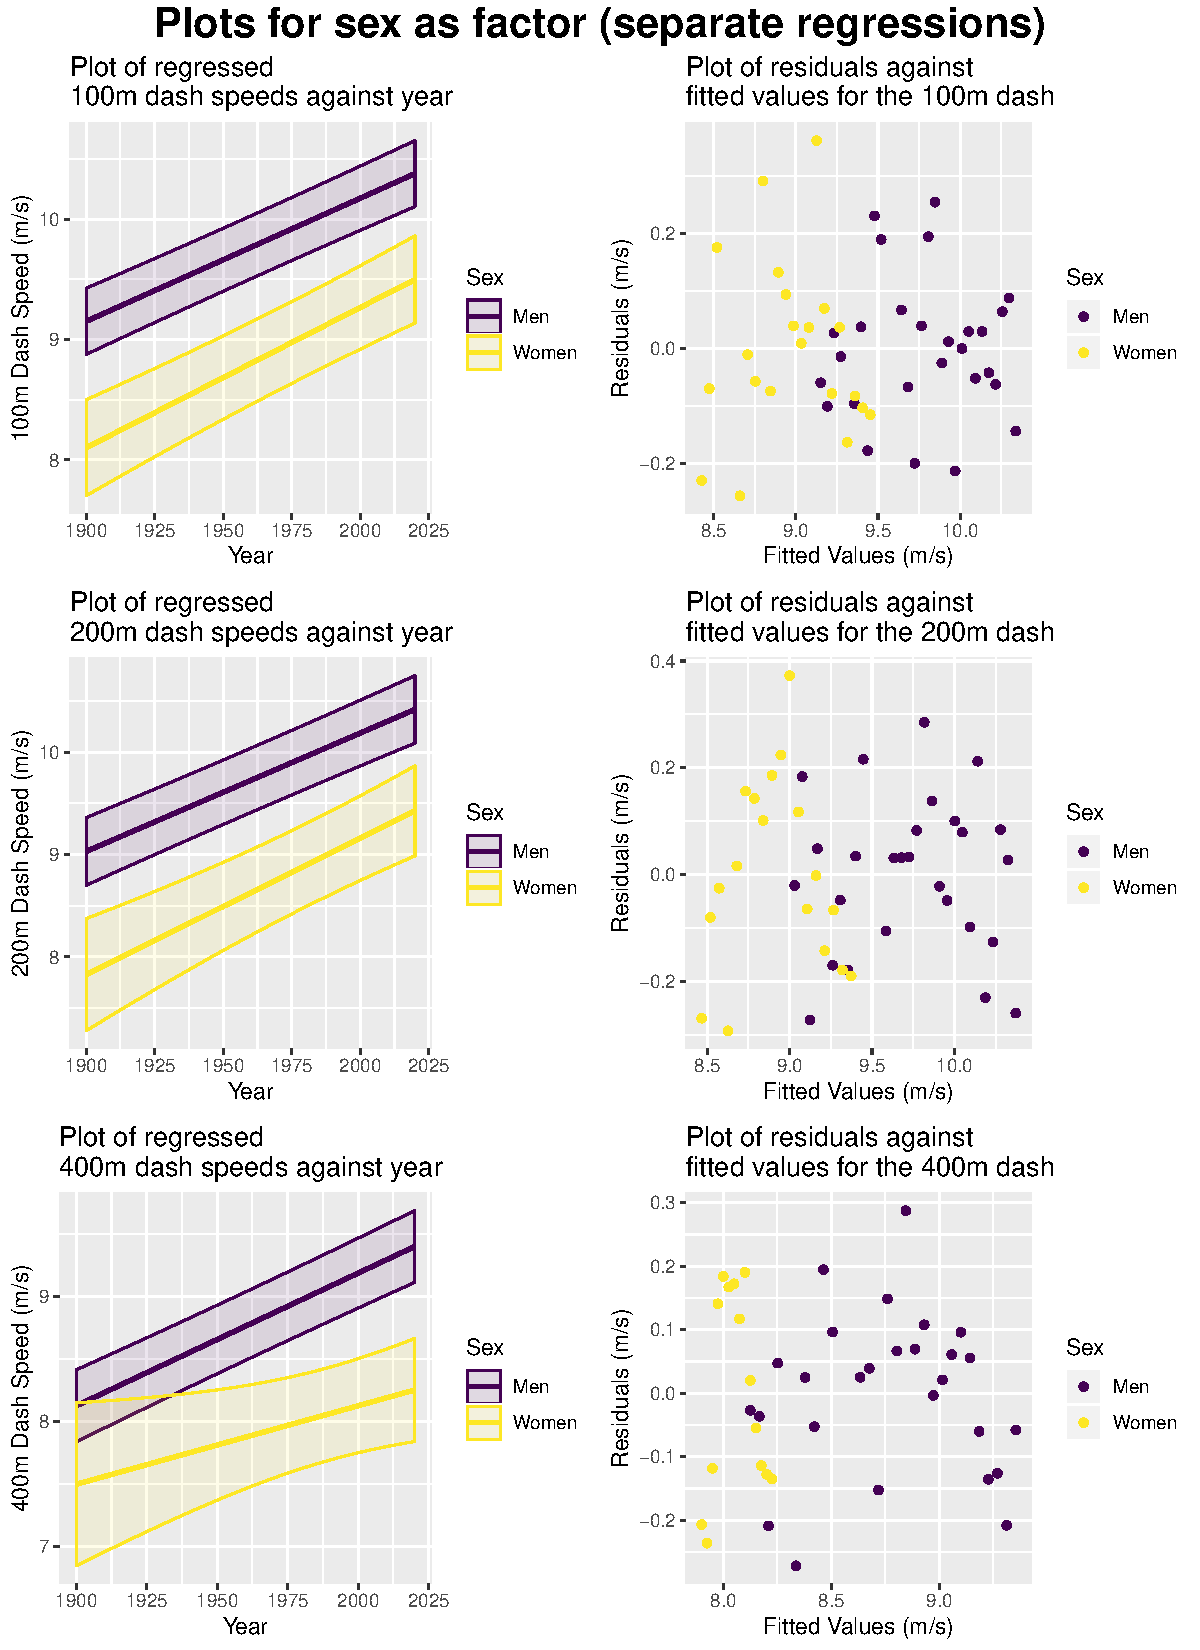
\includegraphics[width=\textwidth]{npplots}
 \caption{Plots showing properties of the separate regressions}
\label{fig:npplots}
\end{figure}

\end{document}